% TeX шаблон, пример оформления отчёта по лабораторной работе.
% Автор: Шмаков И.А.
% Версия от: 05 ноября 2018 года.
% Сборка документа из командной строки:
% ~$ pdflatex -shell-escape main.tex

\documentclass[a4paper,14pt]{extarticle}
\usepackage[utf8]{inputenc}
\usepackage[T2A]{fontenc}
\usepackage[english,russian]{babel}

% одинарный интервал
\usepackage{setspace}
\singlespacing 

\usepackage[left=3cm, right=1cm, top=1.5cm, bottom=1.5cm]{geometry}
\usepackage{icomma} % "Умная" запятая: $0,2$ --- число, $0, 2$ --- перечисление
\usepackage{indentfirst} % Красная строка.

% для гиперссылок и выделение их цветом
\usepackage{xcolor}
\usepackage{hyperref}

 % Цвета для гиперссылок
\definecolor{linkcolor}{HTML}{000000} % цвет ссылок
\definecolor{urlcolor}{HTML}{799B03} % цвет гиперссылок
\hypersetup{pdfstartview=FitH,  linkcolor=linkcolor, urlcolor=urlcolor, colorlinks=true}

% Пакет отвечающий за листинги.
\usepackage[outputdir=build]{minted} 
\renewcommand\listingscaption{Листин}

% Фикс "red box" в minted 
\usemintedstyle{xcode}

% Подключение графики
\usepackage{graphicx}
\usepackage{float}
\DeclareGraphicsExtensions{.png}

\usepackage{amsmath}
\usepackage{nccmath}
\usepackage{mathtools}

\renewcommand{\thesection}{\arabic{section}}

\begin{document}
\begin{titlepage}
  \begin{center}
    \MakeUppercase{Министерство науки и высшего образования Российской Федерации} \\
    \MakeUppercase{ФГБОУ ВО Алтайский государственный университет}
    \vspace{0.25cm}
    
    Физико-технический факультет
    
    Кафедра вычислительной техники и электроники
    \vfill
    
    \textsc{Отчёт по лабораторной работе №2 по курсу \\ <<Практикум по ТРПО>>}
  \bigskip

\end{center}
\vfill

\newlength{\ML}
\settowidth{\ML}{«\underline{\hspace{0.6cm}}» \underline{\hspace{2cm}}}
\hfill\begin{minipage}{0.5\textwidth}
  Выполнил студент 4-го курса, \\ 576 группы:\\
  \underline{\hspace{\ML}} В.\,Е.~Щербаков\\
  «\underline{\hspace{0.7cm}}» \underline{\hspace{2cm}} \the\year~г.
\end{minipage}%
\bigskip

\settowidth{\ML}{«\underline{\hspace{0.6cm}}» \underline{\hspace{2cm}}}
\hfill\begin{minipage}{0.5\textwidth}
  Проверил\\
  \underline{\hspace{\ML}} П.\,Н.~Уланов\\
  «\underline{\hspace{0.7cm}}» \underline{\hspace{2cm}} \the\year~г.
\end{minipage}%
\vfill

\begin{center}
  Барнаул, \the\year~г.
\end{center}
\end{titlepage}

\tableofcontents

\newpage

\section{Введение и постановка задачи}
Необходимо разработать программу для расчета значений семейства функций Бесселя - функции Инфельда и функции Макдональда на языке Haskell.

Программа должна позволять вводить необходимый тип функции, ее порядок и аргумент, и выводить для них значение функции с точностью не хуже десяти знаков после запятой для порядков функции 0, 1 и 2, и с точностью не хуже пяти знаков после запятой для остальных порядков для проверки по таблицам. 

\section{Теоретическое описание задачи}
Для реализации функций Инфельда и Макдональда мы будем использовать формулы разложения в степенной ряд:

\begin{align*}
	I_v = (\frac{z}{2})^v \sum_{k=0}^{\infty} 
	\frac{(\frac{z^2}{4})^k}{k!G(v+k+1)}
\end{align*}

\begin{multline*}
	K_n(z) = \frac{1}{2} (\frac{z}{2})^{-n} \sum_{k=0}^{n-1} 
	\frac{(n-k-1)!}{k!} (\frac{-z^2}{4})^k + (-1)^{n+1} ln \frac{z}{2} + \\
	I_n + \frac{-1^n}{2} (\frac{z}{2})^n \sum_{k=0}^{\infty}
	(\Psi(k+1)+\Psi(n+k+1))) \frac{(\frac{z^2}{4})^k}{k!(n+k)!}
\end{multline*}

где
\begin{align*}
	K_v(z) = \frac{\pi}{2} \frac{I_{-v}(z)-I_v(z)}{sin(\pi v)}
\end{align*}


В этой формуле G - гамма-функция, которая может раскладывать в степенной ряд:
\begin{align*}
	\frac{1}{G(z)} = \sum_{k=1}^{\infty} c_k z^k, |z| < \infty
\end{align*}

\begin{table}[H]
	\centering
	\begin{tabular}{|c|c|}
		\hline
		k & $c_k$ \\
		\hline
		1 & 1 \\
		\hline
		2 & 0.5772156649015329 \\
		\hline
		3 & -0.6558780715202538 \\
		\hline
		4 & -0.0420026350340952 \\
		\hline
		5 & 0.1665386113822915 \\
		\hline
		6 & -0.0421977345555443 \\
		\hline
		7 & -0.0096219715278770 \\
		\hline
		8 & 0.0072189432466630\\
		\hline
		9 & -0.0011651675918591 \\
		\hline
		10 & -0.0002152416741149 \\
		\hline
		11 & -0.0002152416741149 \\
		\hline
		12 & -0.0000201348547807 \\
		\hline
		13 & -0.0000012504934821 \\
		\hline
		14 & 0.0000011330272320 \\
		\hline
		15 & -0.0000002056338417 \\
		\hline
		16 & 0.0000000061160950 \\
		\hline
		17 & 0.0000000050020075 \\
		\hline
		18 & -0.0000000011812746 \\
		\hline
		19 & 0.0000000001043427 \\
		\hline
		20 & 0.0000000000077823 \\
		\hline
		21 & -0.0000000000036968 \\
		\hline
		22 & 0.0000000000005100 \\
		\hline
		23 & -0.0000000000000206 \\
		\hline
		24 & -0.0000000000000054 \\
		\hline
		25 & 0.0000000000000014 \\
		\hline
		26 & 0.0000000000000001 \\
		\hline
	\end{tabular}
\caption{Коэффициенты разложения для $1 <= k <= 26$}
\label{table_1}
\end{table}


Здесь $c_k$ -- коэффициенты разложения (таблица \ref{table_1}). 
Эта формула хорошо аппроксимирует гамму-функцию в отрезке от 1 до 2 с нужной нам точностью. 
Следовательно расчет от большего аргумента должен производиться по рекуррентной понижающей формуле, пока аргумент не попадет в нашу интерполяцию:
\begin{align*}
	G(n+z) = (n - 1 + z)(n - 2 + z) ... (1 + z) G (1 + z)
\end{align*}

При вычислении модифицированных функций Бесселя порядков больше двух или отрицательных нужно воспользоваться рекуррентной формулой:
\begin{align*}
	\zeta_{v-1}(z) - \zeta_{v+1}(z) = \frac{2v}{z} \zeta_v (z)
\end{align*}
где $\zeta_v - I_v$ или $e^{\pi v i} K_v$

Для вычисления функций от большого аргумента могут потребоваться асимптотические разложения:
\begin{align*}
	I_v(z) \frac{e^z}{\sqrt{2 \pi z}} (1 - \frac{(\mu-1)}{8z} + \frac{(\mu-1)(\mu-9)}{2!(8z)^2} - \frac{(\mu-1)(\mu-9)(\mu-25)}{3!(8z)^3} + ...)
\end{align*}

\begin{align*}
	K_v(z) \sqrt{\frac{\pi}{2z}} e^{-z} (1 - \frac{(\mu-1)}{8z} + \frac{(\mu-1)(\mu-9)}{2!(8z)^2} + \frac{(\mu-1)(\mu-9)(\mu-25)}{3!(8z)^3} + ...)
\end{align*}

\section{Проверка работы программы}
Рассчитанные значения для функции Инфельда 0 порядка:
\begin{minted}{text}
	2	2.2795853023360677	0.0
	2.5	3.2898391440501245	0.0
	3	4.880792585865026	0.0
	3.5	7.378203432225482	0.0
	4	11.301921952136334	0.0
	4.5	17.481171855609276	0.0
	5	27.239871823604467	0.0
\end{minted}

Рассчитанные значения для функции Инфельда 1 порядка:
\begin{minted}{text}
	2	1.5906368546373295	0.0
	2.5	2.5167162452886997	0.0
	3	3.9533702174026106	0.0
	3.5	6.205834922258367	0.0
	4	9.759465153704454	0.0
	4.5	15.389222753735929	0.0
	5	24.33564214245053	0.0
\end{minted}

Рассчитанные значения для функции Инфельда 2 порядка:
\begin{minted}{text}
	2	0.6889484476987382	0.0
	2.5	1.2764661478191646	0.0
	3	2.2452124409299525	0.0
	3.5	3.832012048077844	0.0
	4	6.422189375284107	0.0
	4.5	10.641517298393307	0.0
	5	17.505614966624258	0.0
\end{minted}

\begin{figure}[H]
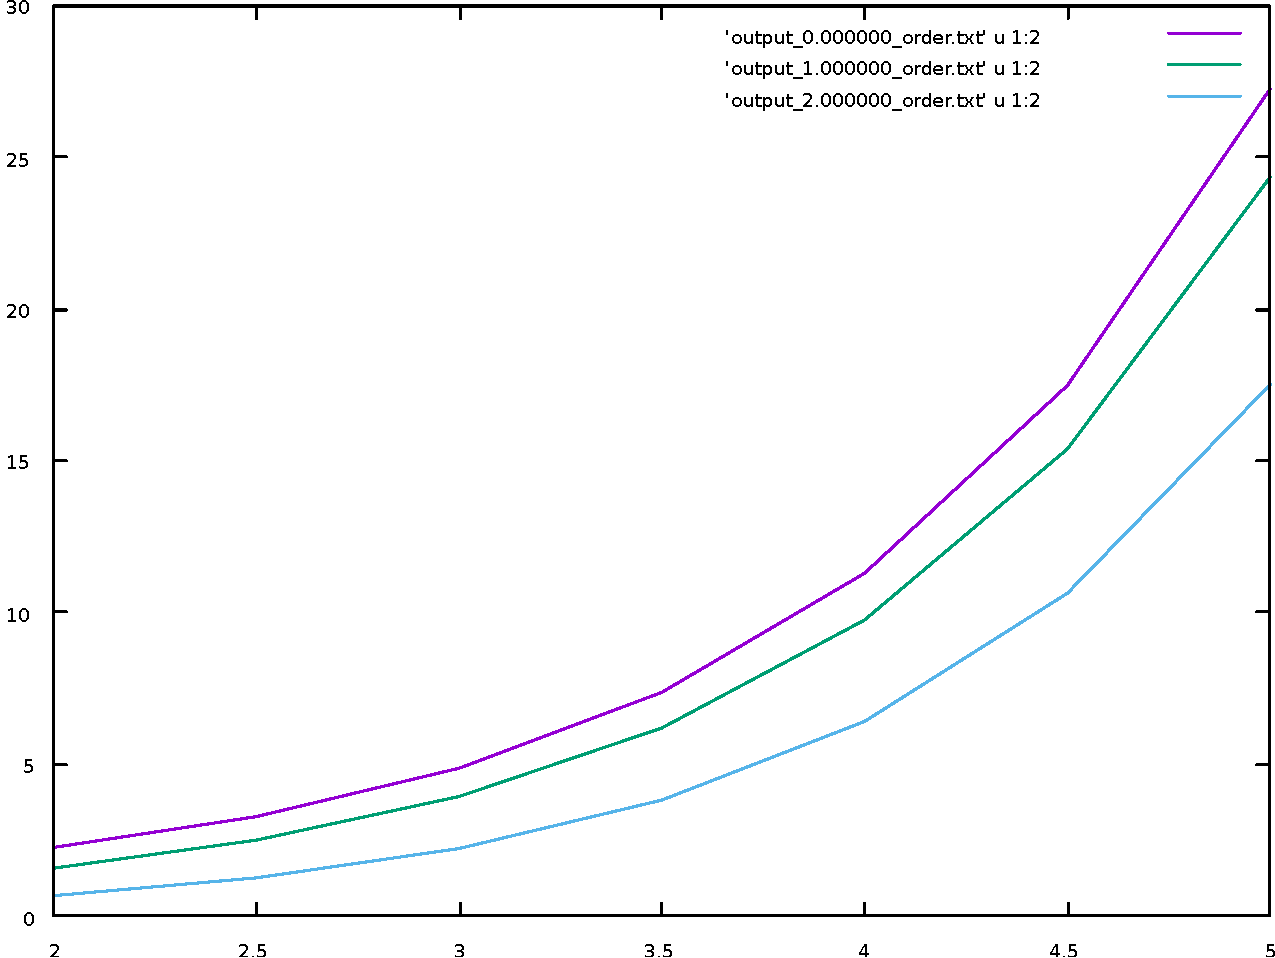
\includegraphics[height=\textwidth, width=\textwidth]{include/inf_1.pdf}
\caption{График функции Инфельда разных порядков}
\end{figure}

\newpage

Рассчитанные значения для функции Макдональда 0 порядка:
\begin{minted}{text}
	0.5	0.9244190712292967	0.0
	1	0.4210244382426492	0.0
	1.5	0.21380556265005018	0.0
	2	0.11389387275302776	0.0
	2.5	6.234755320540897e-2	0.0
	3	3.473950439376061e-2	0.0
	3.5	1.9598897181679398e-2	0.0
	4	1.1159676103171812e-2	0.0
\end{minted}

Рассчитанные значения для функции Макдональда 1 порядка:
\begin{minted}{text}
	0.5	1.6564411200029057	0.0
	1	0.6019072301963682	0.0
	1.5	0.27738780045533895	0.0
	2	0.13986588181408416	0.0
	2.5	7.389081634388939e-2	0.0
	3	4.015643112213407e-2	0.0
	3.5	2.2239392916409972e-2	0.0
	4	1.2483498872311927e-2	0.0
\end{minted}

Рассчитанные значения для функции Макдональда 2 порядка:
\begin{minted}{text}
	0.5	7.550183551240919	3.042206942482102e-8
	1	1.6248388986353854	7.344225946733269e-9
	1.5	0.5836559632571687	2.8627218272685908e-9
	2	0.2537597545671119	1.319800428749823e-9
	2.5	0.12146020628052048	6.59831813833393e-10
	3	6.151045847518333e-2	3.455174458294489e-10
	3.5	3.230712170534224e-2	1.8633186480745733e-10
	4	1.7401425539327775e-2	1.0252844360084282e-10
\end{minted}

\begin{figure}[H]
	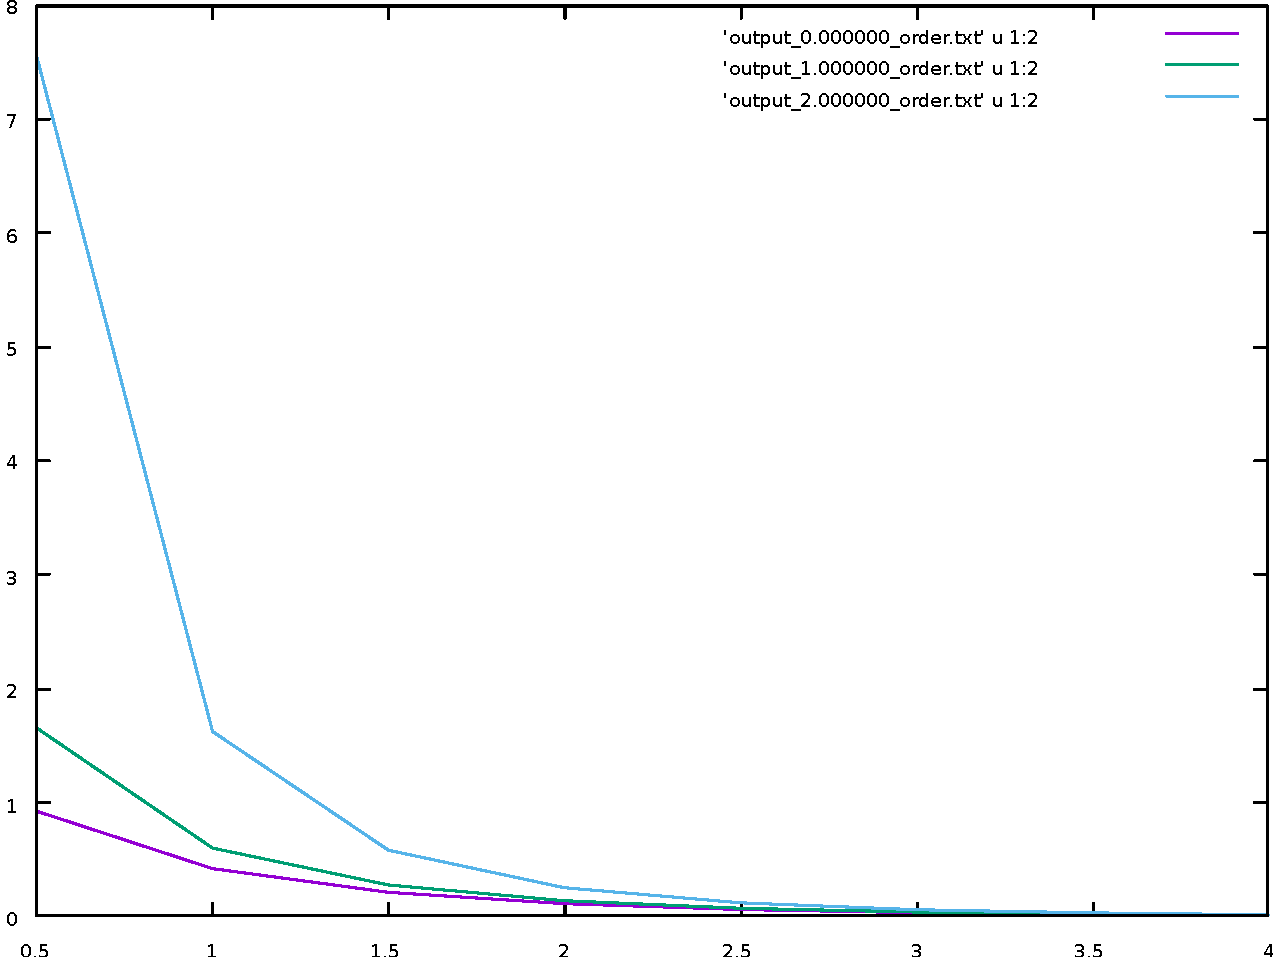
\includegraphics[height=\textwidth, width=\textwidth]{include/macd_2.pdf}
	\caption{График функции Макдональда разных порядков}
\end{figure}

\newpage

Далее построим график зависимости мнимого результата функции Макдональда 1 порядка от фазы и действительного результата от фазы.

\begin{figure}[H]
	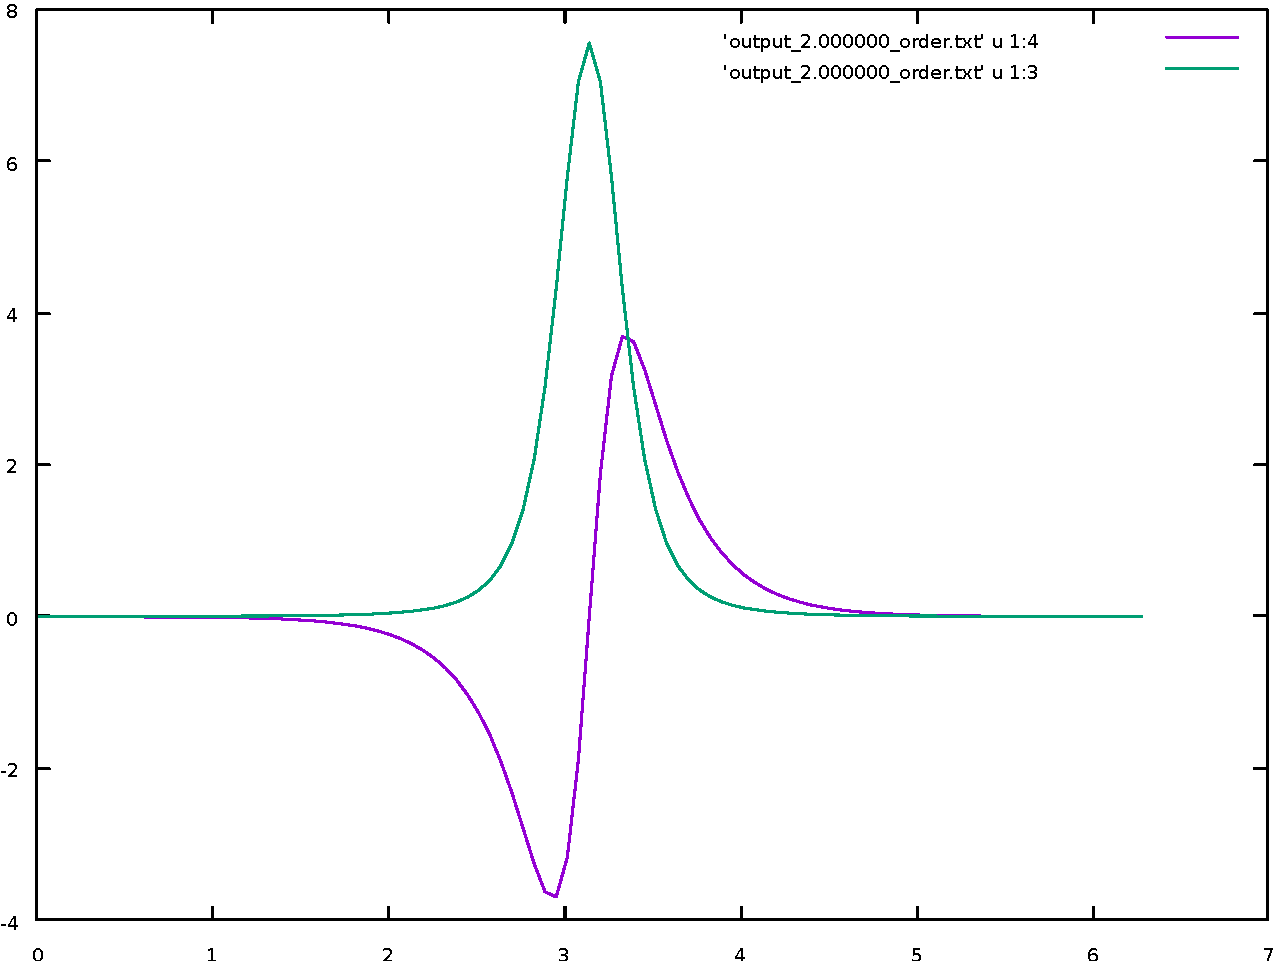
\includegraphics[height=\textwidth, width=\textwidth]{include/mnim_macd.pdf}
	\caption{Зависимость результата функции от фазы}
\end{figure}


\addcontentsline{toc}{section}{Выводы по работе}
\section*{Выводы по работе}
В результате выполнения лабораторной работы были получены навыки программирования на языке Haskell, были изучены особенности функционального подхода.

\newpage

\addcontentsline{toc}{section}{Приложение}
\section*{Приложение}
\inputminted[mathescape,linenos,breaklines]{haskell}{../src/main.hs}

\end{document}          
